\section{Results}

% -------- Part 1: Benchmark
\begin{table}[ht]
\caption{
    \textbf{Benchmark Results.} Test accuracy of all methods on \texttt{TM} and \texttt{SP} in the 5-way-5-shot setting. We depict the average accuracy and the 95\% confidence interval both without (left) and with SOT (right) and the difference.
    \vspace{5pt}
}

\label{tab:tuned-benchmark}
\centering
\begin{tabular}{llllr}
\toprule
 &  & \multicolumn{2}{@{}c}{\textbf{Test Acc. (\%)}} & \\
 &  & w/o SOT & w/ SOT & Diff \\
\midrule
\multirow[c]{5}{*}{\texttt{TM}} & B & $90.7 \pm 0.7$ & $86.3 \pm 0.9$ & {\color{red} +4.8} \\
 & B++ & $81.9 \pm 0.9$ & $82.8 \pm 0.9$ &  {\color{teal} +1.1} \\
 & MAML & $\mathbf{92.8} \pm 0.5$ & $99.2 \pm 0.1$ & {\color{teal} +6.9} \\
 & MN & $84.6 \pm 0.8$ & $\mathbf{99.7} \pm 0.1$ &  {\color{teal} +17.9} \\
 & PN & $87.1 \pm 0.8$ & $98.6 \pm 0.2$ & {\color{teal} +13.2} \\
\midrule
\multirow[c]{5}{*}{\texttt{SP}} & B & $\mathbf{69.2} \pm 0.7$ & $55.7 \pm 0.8$ & {\color{red} -19.6} \\
 & B++ & $64.1 \pm 0.7$ & $64.6 \pm 0.7$ & {\color{teal} +0.8} \\
 & MAML & $68.7 \pm 0.7$ & $98.0 \pm 0.2$ & {\color{teal} +42.8} \\
 & MN & $68.2 \pm 0.8$ & $\mathbf{99.8} \pm 0.1$ & {\color{teal} +46.5} \\
 & PN & $63.5 \pm 0.7$ & $99.2 \pm 0.1$ & {\color{teal} +56.1} \\
\bottomrule
\end{tabular}
\end{table}
Table \ref{tab:tuned-benchmark} displays the results of the first part of 
our benchmark study. We fine-tuned hyper-parameters of each method on the given dataset and 
then evaluated it across 600 episodes. The table presents the mean accuracy,
 accompanied by a 95\% confidence interval across the episodes. 
 The \texttt{Diff} column indicates the change in mean accuracy when we 
 introduce the \texttt{SOT} module to the method.

Firstly, we observe that for the 5-way, 5-shot setting, all methods without 
\texttt{SOT} already reach an average accuracy of 87\% for the \texttt{TM} 
dataset and 66\% for the \texttt{SP} dataset, establishing a very solid baseline performance.
Secondly, we notice that the presence of the \texttt{SOT} module enhances all 
methods except for the Baseline. However, for \texttt{B++}, the performance improvement is only marginal. 
In contrast, for the remaining three methods, \texttt{SOT} improved the performance for the \texttt{TM} dataset 
by an average of 12\% and by 48\% for the \texttt{SP} dataset. 
Therefore, for both datasets, we observe a substantial effect size after the integration of the \texttt{SOT} module.

% -------- Part 2: way-shot analysis
\begin{figure}
    \centering
    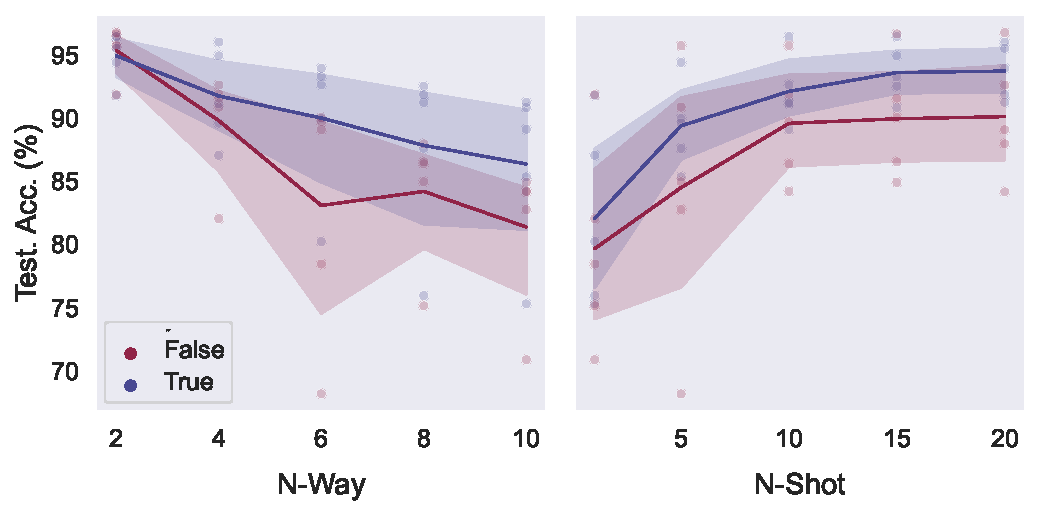
\includegraphics[width=1\columnwidth]{../figures/way-shot.pdf}
    \caption{Accuracy of the Tabula Muris dataset for different ways and shots.}
    \label{fig:way-shot}
\end{figure}


Figure \ref{fig:way-shot} shows the relationship between the number of ways and shots
and the accuracy of the \texttt{ProtoNet} method on \texttt{TM} dataset. 
As we would expect, without the \texttt{SOT} module, the accuracy decreases with the number of ways and 
increases with the number of shots. However, with the \texttt{SOT} module, the accuracy remains 
stable across different ways and shots. 

% -------- Part 3: SOT integration into the matching net
\begin{figure}
    \centering
    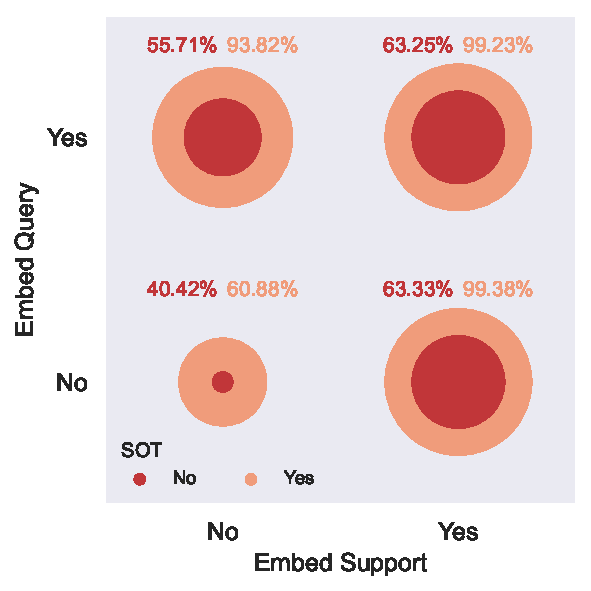
\includegraphics[width=0.75\columnwidth]{../figures/sot-interaction-scatter.pdf}
    \caption{Performane of different configurations of MatchingNet with and without SOT on the Tabula Muris dataset.}
    \label{fig:sot-interaction-scatter}
\end{figure}

In Figure \ref{fig:sot-interaction-scatter}, we illustrate the performance of various 
configurations of the \texttt{MatchingNet} method with and without the \texttt{SOT} 
module. Firstly, it is evident that without any form of embedding, regardless of the presence or 
absence of the \texttt{SOT} module, the performance is only 40\%. Secondly, in the absence of the 
\texttt{SOT} module, the optimal performance is achieved through the embedding of support vectors. 
Slightly inferior performance is observed when the query vectors are embedded. 
Most notably, the \texttt{SOT} module enhances the performance of all configurations. 
However, the optimal performance is attained in configurations where at least one of the 
support or query vectors is embedded.
